\subsection{Flöde vid termisk jämvikt}
\label{sec:steadystatewall}

%To regerenate the figures use /code/pdesolver/generateWallFigApril.m
%with the argument /code/pdesolver/walldata.mat


För att visualisera flödet genom en vägg vid konstant väder och utomhustemperatur görs 
beräkningar med finita elementmetoden och en konstant inomhustemperatur på 
$\unit[20]{^\circ C}$. Utomhusvädret är relativ konstant och är satt till antingen molning 
eller klart och utomhustemperaturen varierar mellan $\unit[6]{^\circ C}$ på natten och 
$\unit[9]{^\circ C}$ på dagen. Detta har gjorts för en vägg utan och en vägg med 
isolering, se figur \ref{fig:energyflow_stst}. Den oisolerade väggen består av 
$\unit[0,5]{m}$ tegel och den isolerade har dessutom $\unit[0,1]{m}$ mineralull. 

\begin{figure}[hpbt]
\centering

\subfloat[Energiflöde ut från insidan av en oisolerad vägg en klar dag.]{
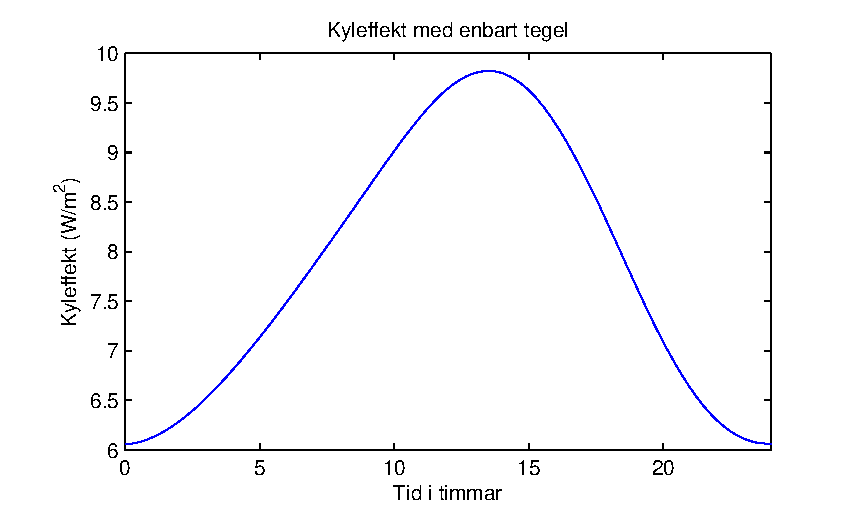
\includegraphics[width=6cm]{images/noinsulationapril.eps}}\vspace{1cm}
\subfloat[Energiflöde ut från insidan av en isolerad vägg en klar dag.]{
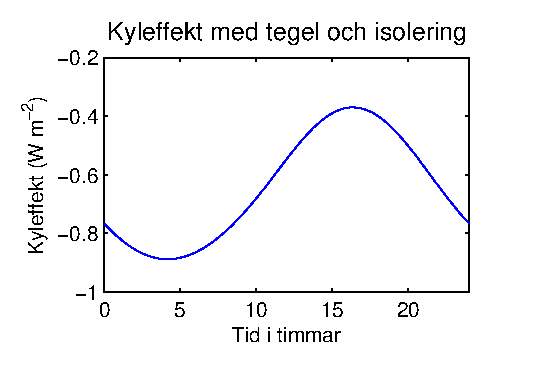
\includegraphics[width=6cm]{images/insulationapril.eps}
}

\subfloat[Energiflöde ut från insidan av en oisoleradvägg en molnig dag.]{
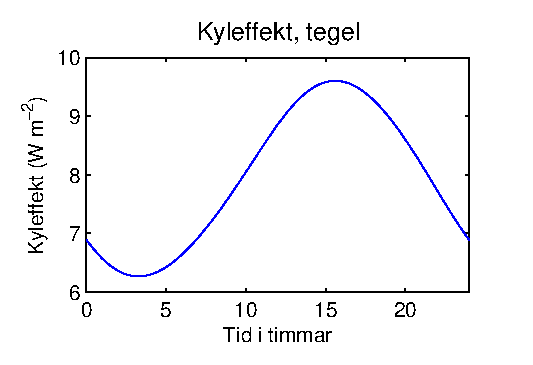
\includegraphics[width=6cm]{images/noinsulationcloud.eps}}\vspace{1cm}
\subfloat[Energiflöde ut från insidan av isolerad vägg en molnig dag.]{
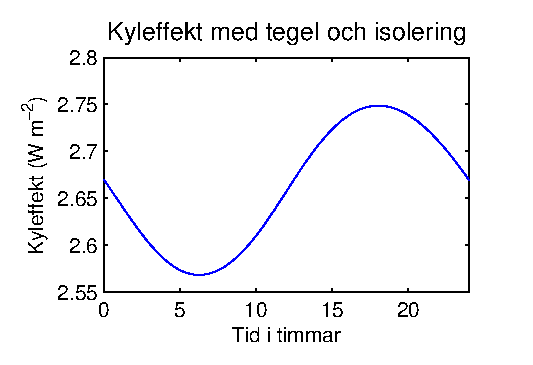
\includegraphics[width=6cm]{images/insulationcloud.eps}
}

\caption{\label{fig:energyflow_stst} Energiflöden ut från insidan av en vägg en dag motsvarande en i mitten av april.
Utomhustemperaturen varierar mellan $\unit[6]{^\circ C}$ på natten och $\unit[9]{^\circ C}$ på dagen. Inomhustemperaturen är satt konstant $\unit[20]{^\circ C}$.}
\end{figure}


%RESULTAT ur graferna 
I figurerna \ref{fig:energyflow_stst} kan vi se att energiflödet genom väggen minskar till 
ungefär en fjärdedel med isolering. Under ett soligt dygn kommer det att flöda värme in i
 fastigheten. På grund av fördröjningen i väggen sker detta främst under natten, 
 och mindre på dagen. Med isolering blir variationen mindre och ett mindre men jämnare 
 energiflöde, under $\unit[1]{W m^{-2}}$, går i fastigheten under hela dygnet.

Under en motsvarande fast molnig dag varierar energiflödet mellan 7 och 10 
$\unit{W m^{-2}}$ till att röra sig mellan 2,1 och 2,3 $\unit{W m^{-2}}$, dock ut ur 
fastigheten. En isolering innebär ett minskat energiutflöde och därmed en minskad 
energiförlust för fastigheten.

Trots att energi flödar in i fastigheten den soliga dygnet så flödar ganska mycket energi 
ut ur fastigheten under det molniga dygnet. Göteborg har 1800 solskenstimmar under ett
 år av de totalt 4380 timmar som solen är över horisonten. Utifrån SMHI:s väderstatistik \cite{SMHIdata}
 kan beräknas att ungefär 37\% av dessa sker under eldningssäsongen, oktober till april. 
 Detta motsvarar ungefär 8\% av dygnets alla timmar. Tyvärr så förlorar fastigheten mer 
 energi än vad den tjänar på att inte isolerat sett till hela eldningssäsongen.

Under en fin sommardag kan det också tänkas att fastigheten värms över den önskade 
temperaturen och energi istället måste läggas på kylning. Med en isolering minskas även 
effekten av detta och energiflödena blir mindre om jämnare.

%%%%%%%%%%%%%%%%%%%%%%%%%%%%%%%%%%%%%%%%%%%%
\paragraph{En decemberdag}

Vidare har också energiflödena genom väggen en kall decemberdag undersökts, 
alltså en dag där energiflödena bör bli ganska stora. Detta kan ses som ett extremfall av
nyår i Göteborg och är då en övre uppskattning på den energiåtgång fastigheten. Två fall av
denna dag har undersökts, dels en molning dag och dels en solig dag.

 Temperaturen går från $\unit[-5]{^\circ C}$ på dagen till $\unit[-11]{^\circ C}$. 
 Konvektionskoefficienten har satts till $h=35$ 
 vilket motsvarar en vindhastighet $\unit[5]{m/s}$ parallellt med väggens yta. 
 Beräkningarna är genomförda genom att väggen approximerats med en stav och 
 därefter behandlats med finita elementmetoden.


\begin{figure}[hpbt]
\centering
\subfloat[Energiflöde en  decemberdag från insidan av en oisolerad vägg en molnig dag]{
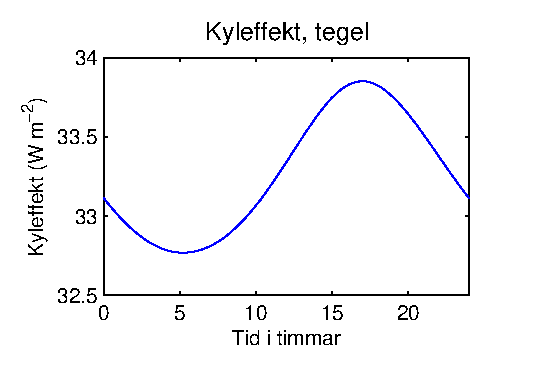
\includegraphics[width=6cm]{images/noinsulationdec.eps}}
\subfloat[Energiflöde från insidan av en isolerad vägg en molnig dag.]{
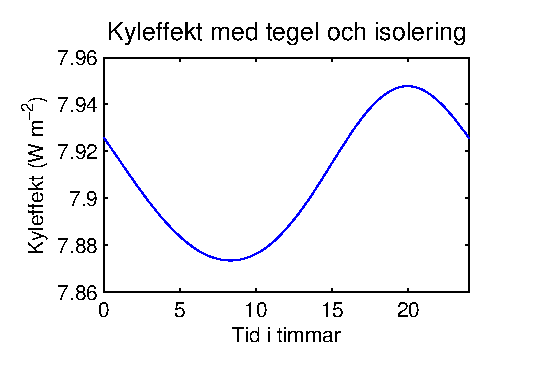
\includegraphics[width=6cm]{images/insulationdec.eps}
}

\subfloat[Energiflöde en solig decemberdag från insidan av en oisolerad vägg]{
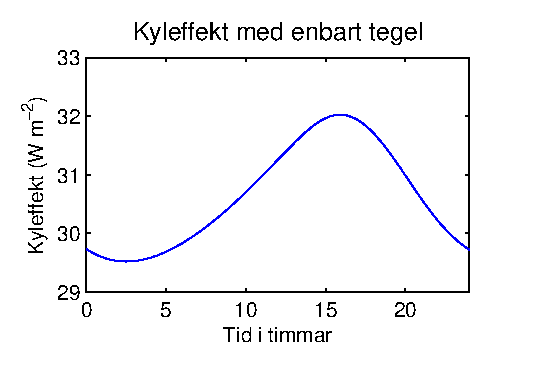
\includegraphics[width=6cm]{images/decsunnoinsulation.eps}
}\vspace{1cm}
\subfloat[Energiflöde en solig decemberdag från insidan av en isolerad vägg]{
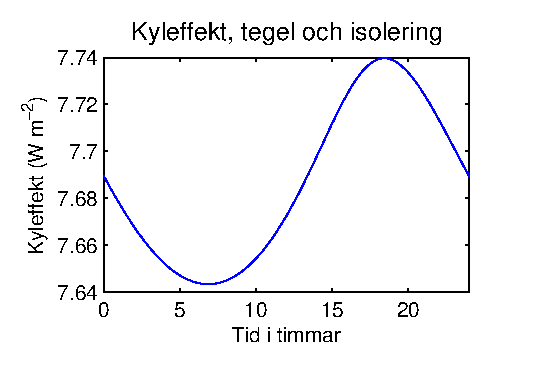
\includegraphics[width=6cm]{images/decsuninsulation.eps}
}

\caption{\label{fig:wall_dec} Energiflöden ut från insidan av en vägg en dag motsvarande en i december.
}
\end{figure}

% Resultat
Även i december blir energiflödet genom en isolerad vägg ungefär en fjädedel av det 
genom en oisolerad dito, se figur \ref{fig:wall_dec}. Här minskar det dock från ungefär 33 
till 7,9 $\unit{W m^{-2}}$ ut ur väggen för den mulna dagen och från ungefär 31 till 7,4 $\unit{W m^{-2}}$ den soliga dagen. Vi ser också i figurerna att energiflödet också blir 
jämnare med isolering – det varierar med mindre än 0,1 $\unit{W m^{-2}}$ över dygnet, 
istället för över 1 $\unit{W m^{-2}}$, utan isolering. Det gäller både med och utan sol. Detta är eftersträvansvärt om en jämn inomhustemperatur önskas. Energiflödet påverkas inte lika mycket av solen på vintern som under den varmare delen av året. Här finns alltså betydligt mindre att tjäna på att inte isolera och hoppas att solen skiner.

%%%% BURSPRÅK %%%%%%%%%%%%%%%%%%%%%%%%%%%%%%%
\paragraph{Burspråket}

Burspråket är inte uppbyggt av tegel, som de andra väggarna, utan av gips, isolering och koppar på spånskiva, se avsnitt \ref{subsec:walls}. Energiflödet i burspråket visas här för alla tre fallen: solig aprildag, molnig aprildag och molnig decemberdag.

\begin{figure}[hpbt]
\centering
\subfloat[\label{fig:bursprak_april1} Energiflödet från insidan av burspråket en klar aprildag.]{
	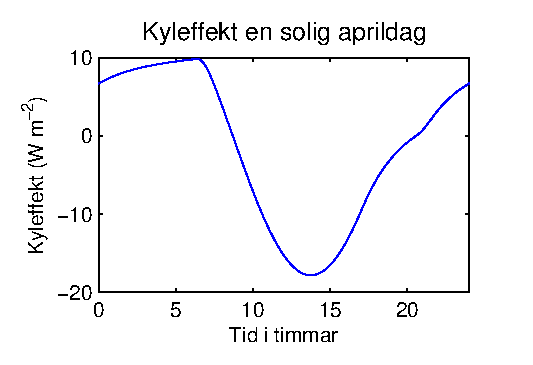
\includegraphics[width=6cm]{images/baysunapril.eps}
}
\subfloat[\label{fig:bursprak_april2} Energiflödet från insidan av burspråket en molnig aprildag.]{
	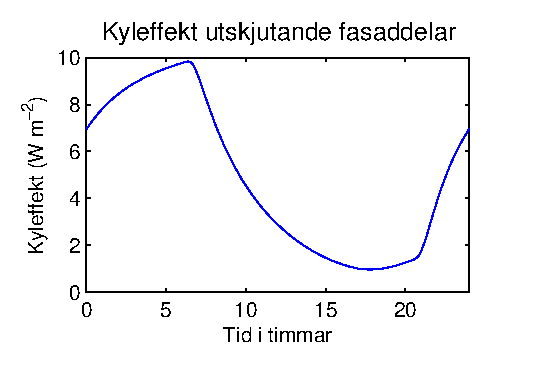
\includegraphics[width=6cm]{images/baynosunapril.eps}
}

\subfloat[\label{fig:bursprak_decsun} Energiflödet från insidan av burspråket en solig decemberdag.]{
  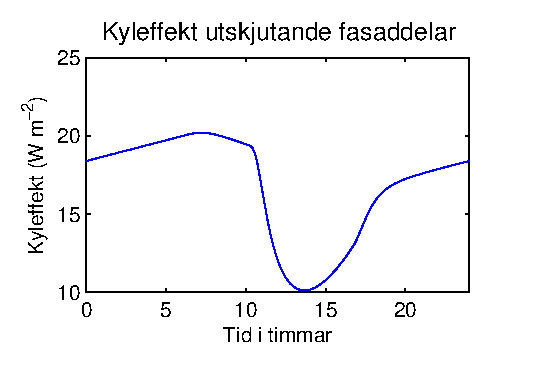
\includegraphics[width=6cm]{images/decsunbay.eps}
}
\subfloat[\label{fig:bursprak_dec} Energiflödet från insidan av burspråket en molnig decemberdag.]{
	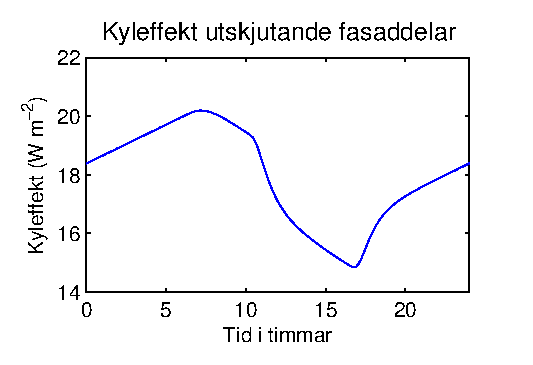
\includegraphics[width=6cm]{images/baynosundec.eps}
}
\caption{\label{fig:bursprak_energi}Energiflödet genom burspråket.}
\end{figure}

Genom burspråket ser energiflödet lite annorlunda ut, figur \ref{fig:bursprak_energi}. En aprilmorgon, innan solen har gått upp, maximeras energiutflödet 10 $\unit{W m^{-2}}$. När solen sedan värmer väggen börjar energi istället flöda in i byggnaden och en riktigt solig dag är det maximala inflödet nästan 20 $\unit{W m^{-2}}$, se figur \ref{fig:bursprak_april1}. En molnig dag stannar det istället på ungefär 1 $\unit{W m^{-2}}$ ut ur väggen, se figur \ref{fig:bursprak_april2}

 En molnig dag  i december är det betydligt kallare och energiutflödet varierar mellan 15 och 20 $\unit{W m^{-2}}$, se figur \ref{fig:bursprak_dec}. En solig decemberdag är det tyvärr inte mycket bättre och kyleffekten är alltid större än $\unit{W m^{-2}}$, se figur \ref{fig:bursprak_decsun}.
 En intressant detalj är att kyleffekten på burspråket inte alls är sinusformad, så som flödet genom väggarna i figur \ref{fig:energyflow_stst} och \ref{fig:wall_dec}. Det beror troligen på att väggen är väldigt tunn och reagerar snabbt på olika förändringar.

%%%%%%%%TAKET%%%%%%%%%%%%%%%%%%%%%%%%%%%%%%%
\paragraph{Taket}

Energiflödet genom taket beräknas på samma sätt som energiflödet genom väggarna. Skillnaden, förutom materialet, är takets vinkel mot solen. I figur \ref{fig:rooffiguressun} visas energiflödet för en solig april- respektive decemberdag. Eftersom taket lutar har nordsidan och sydsidan olika flöden ty solen skiner olika mycket på de olika lutade ytorna. Figur \ref{fig:rooffigurescloud} visar i sin tur situationen på molniga dagar, då ingen direkt solstrålning faller på taket.

\begin{figure}[hpbt]
\centering
\subfloat[\label{fig:roofaprilsunsouth} Energiflöde från insidan av sydsidan på taket en klar aprildag.]{
	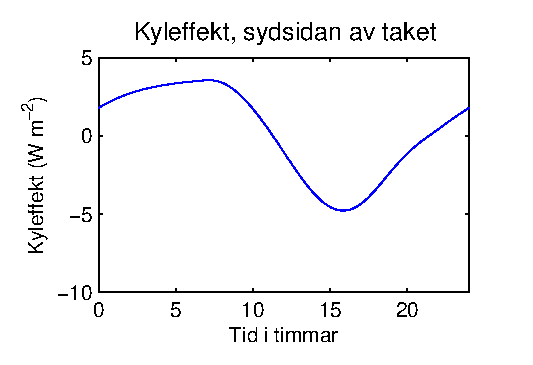
\includegraphics[width=6cm]{images/roofaprilsunsouth.eps}
}
\subfloat[\label{fig:roofaprilsunnorth} Energiflöde från insidan av norrsidan på taket en klar aprildag.]{
	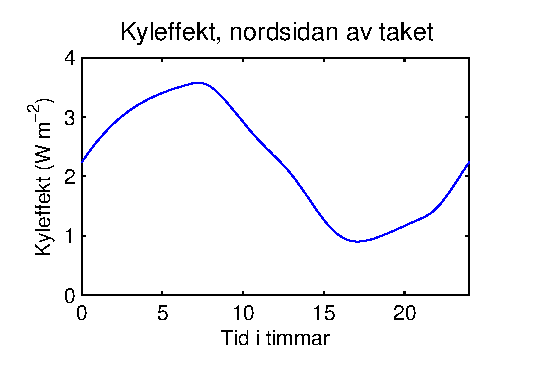
\includegraphics[width=6cm]{images/roofaprilsunnorth.eps}
}

\subfloat[\label{fig:roofdecsunsouth} Energiflödet från insidan av sydsidan på taket en klar decemberdag.]{
	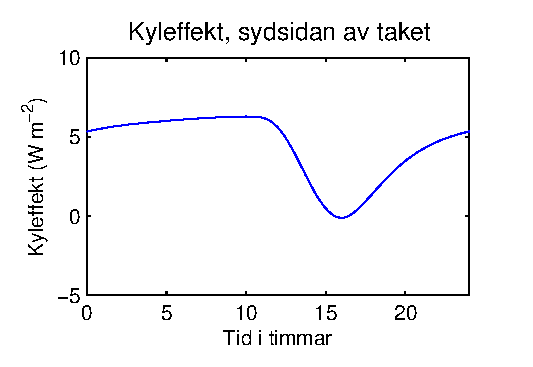
\includegraphics[width=6cm]{images/roofdecsunsouth.eps}
}
\subfloat[\label{fig:roofdecsunnorth} Energiflödet från insidan av nordsidan på taket en klar decemberdag.]{
	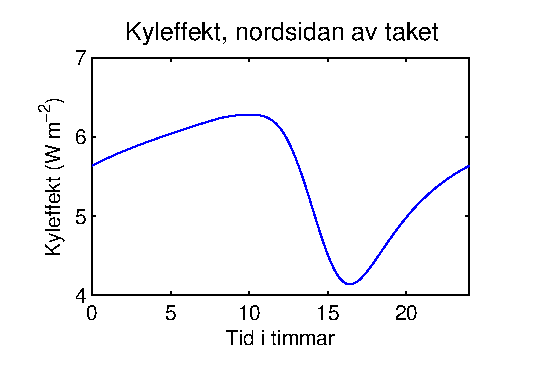
\includegraphics[width=6cm]{images/roofdecsunnorth.eps}
}

\caption{\label{fig:rooffiguressun}Energiflödet genom taket, soliga dagar.}
\end{figure}

\begin{figure}[hpbt]
\centering
\subfloat[\label{fig:roofaprilnosun} Energiflödet från insidan av taket en molnig aprildag.]{
	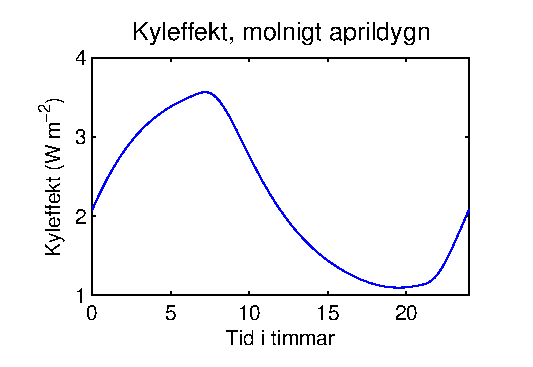
\includegraphics[width=6cm]{images/roofaprilnosun.eps}
}
\subfloat[\label{fig:roofdecnosun} Energiflödet från insidan av taket en molnig decemberdag.]{
	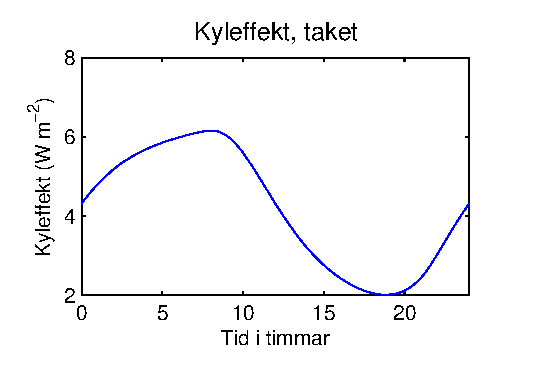
\includegraphics[width=6cm]{images/roofdecnosun.eps}
}

\caption{\label{fig:rooffigurescloud}Energiflödet genom taket, molniga dagar.}
\end{figure}

Energiflödet genom taket en solig dag i april varierar mellan $\unit[5]{W m^{-2}}$ in och $\unit[4]{W m^{-5}}$ ut på sydsidan, se figur \ref{fig:roofaprilsunsouth}, och mellan 1 och $\unit[3]{W m^{-2}}$ ut på nordsidan, se figur \ref{fig:roofaprilsunnorth}. Detta kan vidare jämföras med en molnig aprilldag där utflödet varierar ytterligare lite mindre, bara mellan 1 och $\unit[3,5]{W m^{-2}}$, se figur \ref{fig:roofaprilnosun}. Solen har alltså stor påverkan på energiflödets variationer. En dag i december är energiutflödet endast något högre och varierar mellan 6 och $\unit[4]{W m^{-2}}$, se figur \ref{fig:roofdecnosun},


%%%%%%%%%%%%%%%%%%%%%%%%%%%%%%%%%%%%%%%%%%%%
